\section{Architectural Conformance}

This section applies architectural conformance against a fixed six-point checklist, used consistently for both parts regardless of when it was formally introduced. Part 1's process checked only two of the six points --- single-responsibility violations and unintended coupling between modules --- and did so occasionally, as problems surfaced, rather than by rule. Part 2 extended checking to the remaining four points --- untested code paths, excessive prop-drilling, unused or dead state, and inconsistent naming --- and applied all six by rule, for every feature, through its Post-Implementation Review Agent.

Part 1's two documented cases show what "occasionally, as problems surfaced" meant in practice. The MainPage.js monolith is a direct single-responsibility violation: at 186 lines it already owned three distinct regions --- the top bar, the sidebar, and the main panel --- before the remaining planned features had even been implemented. The missing service layer and the scattered authentication-state reads are both instances of unintended coupling: components were tightly bound to their own fetch logic and their own direct reads of local storage, rather than depending on one shared place for either concern.

Part 2 checked all six categories for every feature, by rule, through the Post-Implementation Review Agent's review\_report.md, which rates each of the six concerns individually and closes with an overall verdict before a human decides whether to fix, defer, or accept. The four categories Part 1 never checked --- untested code paths, excessive prop-drilling, unused or dead state, and inconsistent naming --- only became part of architectural conformance with Part 2's checklist. The review recorded for the workspace-level roles feature shows all six points checked together for one feature, reproduced in \Cref{fig:review-report-checklist}.

\begin{figure}[H]
    \centering
    \begin{subfigure}[b]{0.48\linewidth}
        \centering
        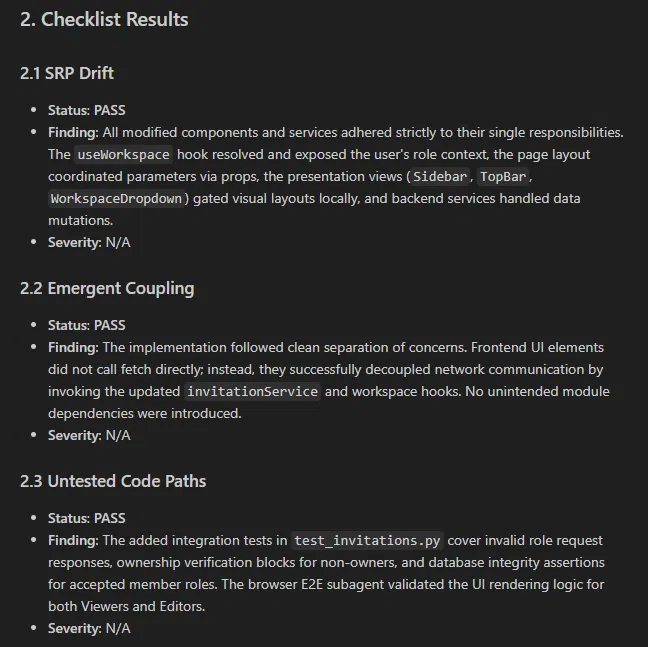
\includegraphics[width=\linewidth]{Bilder/Evaluation/2.1-2.3.png}
    \end{subfigure}
    \hfill
    \begin{subfigure}[b]{0.48\linewidth}
        \centering
        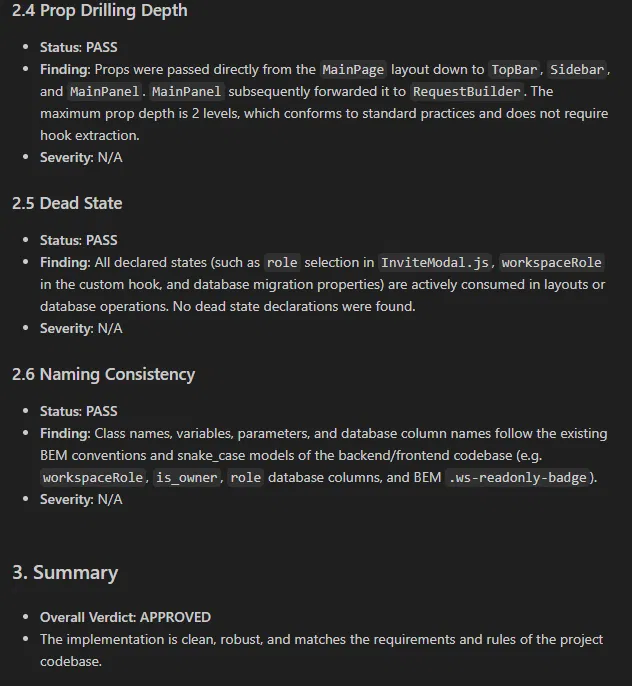
\includegraphics[width=\linewidth]{Bilder/Evaluation/2.4-2.6.png}
    \end{subfigure}
    \caption{Post-Implementation Review Agent's six-point architectural checklist for the workspace-level roles feature, recorded in review\_report.md.}
    \label{fig:review-report-checklist}
\end{figure}

Taken together, Part 1's conformance checking covered two of the six categories, both caught only once already widespread. Part 2's conformance checking covers all six, by rule, and the workspace-roles review shows it actually happening in full for one feature, not only guaranteed in principle.

